\documentclass[11pt,a4paper,english]{article}
\usepackage[latin1]{inputenc}
\usepackage[T1]{fontenc}
\usepackage{t1enc}

% Latex report template for The Norwegian Meteorological Institute
% Updated 2013-06-10 by Oskar Landgren, oskar.landgren@met.no
% Edit as you wish, but please report if you find any errors. 

% Lines starting with "%% LPR: ..." explains what is added 
% or changed by Lars Petter Røed (LPR, larspr@met.no)

\usepackage[english]{babel}
%% LPR: Changed graphic package. Note that pstricks is in conflict with 
%       package xcolor
\usepackage{graphicx}
%\usepackage{epsfig}		% To allow figures
\usepackage{pstricks}		% To draw color pictures directly

\usepackage{fancyhdr}
\usepackage[verbose,a4paper,tmargin=30mm,bmargin=37.5mm,lmargin=30mm,rmargin=30mm]{geometry}

%% LPR: Packages amssymbol and amsmath added to make use of extended
%       special and mathematical characters, e.g., bold greek letters        
\usepackage{amssymb}		% More special characters          
\usepackage{amsmath}		% More mathematical characters

%% LPR: The packages natbib added to ease referencing. Remember to 
%       specify the pathway where to find the bib-file (the file 
%       containing the references) at the location where you wish the
%       the reference chapter to appear (see near the end of this file). 
\usepackage{natbib}			% References

%% LPR: The package multirow added to allow for multiple rows
\usepackage{multirow}

%% LPR: Package verbatim added to allow use of \begin{comment} and \end{comment}
%       environment
\usepackage{verbatim}		% Use the verbatim styles
\usepackage{moreverb}		% Use the moreverb styles
\usepackage{hhline}			% Helps to do lines in tables
\usepackage{colortbl}		% To enable coloring table cells
\usepackage{listings}		% To enable use of dinglings 
\usepackage{graphics}		% is needed for \includegraphics
    
% The new visual identity uses Arial as main font. It is not a free font so 
% it may not be included in your Linux installation.
% Here we use the uarial package, which can be installed using: 
% sudo getnonfreefonts-sys -a

%\usepackage{uarial}
% Another similar sans-serif font is Helvetica:
\usepackage{helvet}

% Required lines for Arial:
%\renewcommand{\familydefault}{\sfdefault}
\renewcommand{\rmdefault}{phv}
\renewcommand{\sfdefault}{phv}

\usepackage{rotating}

% These packages were used before, but I could not find them in my TeX installation.
%\usepackage{publication} 
%\usepackage{tellus} 

% The following puts section numbers in the margin. Comment it if not needed.
% (see example at http://www.howtotex.com/tips-tricks/section-numbering-in-margins/ )
%% LPR: Commented the next line, since it is in conflict with package pstricks 
%\usepackage[usenames,dvipsnames]{xcolor}
\makeatletter
\def\@seccntformat#1{\llap{\csname the#1\endcsname\quad}}
\makeatother
% end of margin numbering

\definecolor{METblue}{cmyk}{0.85,0,0.2,0.2}
%% LPR: Added som new colorcoding
\definecolor{Bluea}{cmyk}{.20,0,0,0}
\definecolor{Blueb}{cmyk}{.40,0,0,0}
\definecolor{Bluec}{cmyk}{.60,0,0,0}
\definecolor{Blued}{cmyk}{.80,0,0,0}
\definecolor{Bluee}{cmyk}{1.0,0,0,0}

%\listfiles
%\renewcommand{\baselinestretch}{1.33}
\renewcommand{\baselinestretch}{1.1}
% \geometry{verbose,a4paper,tmargin=20mm,bmargin=20mm,lmargin=30mm,rmargin=30mm}

%% LPR: The following 12 items are my definitions/abbreviations to ease the
%       writing 

% 1. Often used names 

% 2. Begin and end commands
\def\be{\begin{equation}}
\def\ee{\end{equation}}
\def\beq{\begin{eqnarray}}
\def\eeq{\end{eqnarray}}
\def\bequ{\begin{eqnarray*}}
\def\eequ{\end{eqnarray*}}

% 2.3 Numerical time step and grid steps:
\def\Dx{\Delta x}
\def\Dy{\Delta y}
\def\Dz{\Delta z}
\def\Dt{\Delta t}
\def\Ds{\Delta s}

% 3. Miscellaneous
\newcommand{\husk}[1]{\marginpar{\fbox{#1}}} %Gir feilmelding i margen
\def\phv{\fontfamily{phv}\selectfont}
%\def\nl{\newline}
\def\half{\frac{1}{2}}

% 5. Ordinary derivatives
\def\pt{\partial_t}
\def\px{\partial_x}
\def\py{\partial_y}
\def\pz{\partial_z}
\def\del{\nabla}

% 6. General coordinate derivatives
\def\ptt{\partial_{t'}}
\def\pxt{\partial_{x'}}
\def\pyt{\partial_{y'}}
\def\pzt{\partial_{s}}
\def\delt{\nabla_s}

% 7. Rho or isopycnal coordinate derivatives
\def\ptr{\partial_{t'}}
\def\pxr{\partial_{x'}}
\def\pyr{\partial_{y'}}
\def\pzr{\partial_{\rho}}
\def\delr{\nabla_{\rho}}

% 8. Sigma coordinate derivatives
\def\pts{\partial_{t'}}
\def\pxs{\partial_{x'}}
\def\pys{\partial_{y'}}
\def\pzs{\partial_{\sigma}}
\def\dels{\nabla_{\sigma}}

% 9. Often used vectors
\def\bu{\mathbf u}
\def\bi{\mathbf i}
\def\bj{\mathbf j}
\def\bk{\mathbf k}
\def\vec{\mathbf}

% 10. Mean quantities
\def\meanu{\hat{\mathbf u}}
\def\meanD{\overline{D}}
\def\meanw{\overline{\omega}}
\def\meanrho{\hat{\rho}}
\def\meanp{\overline{p}}
\def\meaneta{\overline{\eta}}
\def\meaneps{\hat{\epsilon}}

% 11. Often used abbreviations
\def\HL{\textsf{HIRLAM}}
\def\RO{\textsf{ROMS}}
\def\ROH{\textsf{HIROMS}}
\def\SV{\textsf{SVIM4}}
\def\MI{\textsf{MIPOM}}
\def\B2{\textsf{BaSIC2}}
\def\B4{\textsf{BaSIC4}}
\def\yr{\textsf{http://www.yr.no}}
\def\Basic{\textsf{BaSIC}}
\def\FB{Fugl{\o}ya - Bj{\o}rn{\o}ya}

% 12. Often used quantities
\def\Ds{\Delta s}
%\def\PTV{\mathcal{Q}}
%\def\trho{\tilde{\rho}}

%% LPR: End my definitions

%% LPR: Replaced the ams bibliography style by agufull04
%\bibliographystyle{ams} 
\bibliographystyle{agufull04}
%\bibliographystyle{/home/larspr/LATEX/bst-files/agufull04}

%% LPR: New size and headname for figures and tables
\renewcommand{\figurename}{\footnotesize{Fig.}}
\renewcommand{\tablename}{\footnotesize{Table}}

%% LPR: Added the path to figures and plots
\graphicspath{{./GRAPHICS/}}


\begin{document}

\thispagestyle{empty}

\noindent
\begin{tabular}{@{} p{63mm} p{50mm} r}
\includegraphics*[]{met_rapport_logo_eng}
& {\Huge \bf MET {\color{gray} report} } &
 \begin{minipage}[b]{28mm}
  \begin{flushright}

%% LPR: Changed Topic to Oceanography
   \footnotesize no. 23/2014 \\ Oceanography              % Report number and
   % Topic
  \end{flushright}
 \end{minipage}
\end{tabular}

%\vfill

\begin{flushright}
{ \huge \bf BaSIC Technical Report 3:}
% Title

% Optional subtitle here:
\vspace{2mm}
{ \Large \bf Evaluation of the BaSIC20 long term hindcast results}

\vspace{5mm} 

% Author(s) name
Lars Petter R{\o}ed\footnote{Norwegian Meteorological Institute, R\&D Department, Norway}$^,$\footnote{Institute of Geosciences, University of Oslo}, Vidar Lien$^3$, Arne Melsom$^1$, Nils Melsom Kristensen$^1$, Yvonne Gusdal$^1$ and Bj{\o}rn {\AA}dlandsvik\footnote{Institute of Marine Research, Norway}
\end{flushright}

\vspace{2mm}

\begin{figure}[!h]
 \begin{center}
 % \includegraphics*[width=12cm]{DeltaT_2005-2009_upper100m.png}          %
  \includegraphics*[width=15cm]{./GRAPHICS/Fra_Nils_2014-07-25/b20kpp_25y_mean_85-09_energy.png}         
  % Graphic
 \end{center}
\end{figure}

%% LPR: Added command to add an empty page
%\clearpage
\newpage
\thispagestyle{empty}
\noindent \textbf{\color{white} aa} 

\setlength{\unitlength}{1mm}  % Needed for picture environment

\newpage
\thispagestyle{empty}

\begin{table}[!ht]

\begin{tabular}[c]{lr}
 \vspace{5mm}
 \includegraphics*{met_rapport_logo_eng} & \hspace{70mm}
 {\Huge \bf MET {\color{gray} report} } \\
\end{tabular}

\newpage
\thispagestyle{empty}

\begin{tabular}[t]{|p{110mm}|p{40mm}|} \hline
 {\bf Title}                  & {\bf Date}               \\ 
 %Title goes here
 BaSIC Technical Report 3: Evaluation of the BaSIC20 long term hindcast results & August 30, 2014 %\today               
 \\ \hline {\bf Section}                & {\bf Report no.}         \\ 
  Ocean and Ice                        &  23/2014                  \\ \hline
 {\bf Author(s)}                 & {\bf Classification}     \\ 
 %Author(s) name
 Lars Petter R{\o}ed, Vidar Lien, Arne Melsom, Nils Melsom Kristensen, Yvonne Gusdal and
Bj{\o}rn {\AA}dlandsvik               
                             & \begin{picture}(20,4)(-2,-1.0)
                               \put (0,0){\circle{4}}
                               \put (7,0){\makebox(0,0){Free}}
                               \put (15,0){\circle*{4}}
                               \put (27,0){\makebox(0,0){Restricted}}
                               \end{picture}
                               \\ \hline
 {\bf Client(s)}              & {\bf Client's reference} \\ 
 %Client name                  &               \\ \hline
 Statoil                  & Contract: 4502465983  \\ \hline
\end{tabular}

\begin{tabular}[t]{|p{154mm}|}
{\bf Abstract}                                          \\ 
%Abstract text...
Provided is documentation of a new Oslofjord model, FjordOs CL, utilizing the curvilinear option of the Regional Ocean Modeling System - ROMS. The development is part of the project FjordOs. FjordOs CL has a spatial grid size varying from about 50 meters in the {\DR} sound to about 300 meters at its southern open boundary bordering on the Skagerrak. It features 42 terrain-following levels in the vertical. In addition to being forced by atmospheric, river and tidal input it is also forced by oceanic input at the open boundary. The atmospheric input is extracted from MET Norway's operational NWP model (AROME-MetCoOp), while oceanic input is extracted from MET Norway's operational, ocean forecasting model NorKyst800. The river input consists of observational based estimated discharges from 37 rivers along the perimeter of the fjord. The tidal input is based on the TPXO Atlantic database modified by observations and consists of nine tidal constituents as input.

\vfill
\\ \hline
{\bf Keywords}                                          \\ 
Oceanography, Numerical Modeling, Ocean Climate, Arctic and Nordic Seas \\ 
                                                        \\
\hline
\end{tabular}

\begin{tabular}[t]{cc}
                             &                            \\
                             &                            \\
                             &                            \\
\line(1,0){70}               & \line(1,0){70}             \\ 
Disciplinary signature       & Responsible signature      \\
Lars Anders Breivik          & {\O}ystein Hov                \\       % Add names if needed
\hspace{75mm}                & \hspace{75mm}              \\

\end{tabular}
\end{table}

%\newpage
\thispagestyle{fancy} % footer from fancyhdr package
\headheight=15pt
\renewcommand{\headrulewidth}{0pt}

\begin{comment}
\begin{abstract}
 Provided is documentation of a new Oslofjord model, FjordOs CL, utilizing the curvilinear option of the Regional Ocean Modeling System - ROMS. The development is part of the project FjordOs. FjordOs CL has a spatial grid size varying from about 50 meters in the {\DR} sound to about 300 meters at its southern open boundary bordering on the Skagerrak. It features 42 terrain-following levels in the vertical. In addition to being forced by atmospheric, river and tidal input it is also forced by oceanic input at the open boundary. The atmospheric input is extracted from MET Norway's operational NWP model (AROME-MetCoOp), while oceanic input is extracted from MET Norway's operational, ocean forecasting model NorKyst800. The river input consists of observational based estimated discharges from 37 rivers along the perimeter of the fjord. The tidal input is based on the TPXO Atlantic database modified by observations and consists of nine tidal constituents as input.
    % Abstract text here ...
\end{abstract}
\end{comment}

%\vfill

\fancyfoot{
% If abstract on separate page is not needed, move the following table to the page before
\begin{tabular}[b]{p{28mm}p{28mm}p{28mm}p{28mm}p{28mm}}
 \begin{minipage}[l]{28mm} \tiny \color{METblue} {\bf Meteorologisk institutt}\\ Meteorological Institute\\ Org.no 971274042\\ post@met.no
 \end{minipage} & 
 \begin{minipage}[l]{28mm} \tiny \color{METblue} {\bf Oslo}\\ P.O. Box 43 Blindern\\ 0313 Oslo, Norway\\ T. +47 22 96 30 00
 \end{minipage} &
 \begin{minipage}[l]{28mm} \tiny \color{METblue} {\bf Bergen}\\ All\'egaten 70\\ 5007 Bergen, Norway\\ T. +47 55 23 66 00
 \end{minipage} & 
 \begin{minipage}[l]{28mm} \tiny \color{METblue} {\bf Troms{\o}}\\ P.O. Box 6314\\ 9293 Troms{\o}, Norway\\ T. +47 77 62 13 00
 \end{minipage} & 
 \begin{minipage}[l]{28mm} \tiny \color{METblue} www.met.no\\ www.yr.no
 \end{minipage}
\end{tabular}
}

%% LPR: Added command to add an empty page
\newpage
\thispagestyle{empty}
\noindent \textbf{\color{white} aa} 

%% LPR: Moved abstract up before Table of Contents
%\clearpage


\begin{comment}
\fancyfoot{
% If abstract on separate page is not needed, move the following table to the page before
\begin{tabular}[b]{p{28mm}p{28mm}p{28mm}p{28mm}p{28mm}}
 \begin{minipage}[l]{28mm} \tiny \color{METblue} {\bf Meteorologisk institutt}\\ Meteorological Institute\\ Org.no 971274042\\ post@met.no
 \end{minipage} & 
 \begin{minipage}[l]{28mm} \tiny \color{METblue} {\bf Oslo}\\ P.O. Box 43 Blindern\\ 0313 Oslo, Norway\\ T. +47 22 96 30 00
 \end{minipage} &
 \begin{minipage}[l]{28mm} \tiny \color{METblue} {\bf Bergen}\\ All\'egaten 70\\ 5007 Bergen, Norway\\ T. +47 55 23 66 00
 \end{minipage} & 
 \begin{minipage}[l]{28mm} \tiny \color{METblue} {\bf Troms{\o}}\\ P.O. Box 6314\\ 9293 Troms{\o}, Norway\\ T. +47 77 62 13 00
 \end{minipage} & 
 \begin{minipage}[l]{28mm} \tiny \color{METblue} www.met.no\\ www.yr.no
 \end{minipage}
\end{tabular}
}
\end{comment}

%% LPR: Added an empty page
%\newpage
%\thispagestyle{empty}
%\noindent \textbf{\color{white} aa} 

%\newpage
\clearpage
\pagenumbering{roman} % Use roman numerals for page numbering before main content.
%\thispagestyle{empty} % Hide page numbers
\tableofcontents 

%% LPR: Added an empty page before List of tables and figures
\newpage
\thispagestyle{empty}
\noindent \textbf{\color{white} aa}

%% LPR: Added a list of Tables beginning on a new page
\newpage
\listoftables

%% LPR: Added an empty page before List of Figures
\newpage
\thispagestyle{empty}
\noindent \textbf{\color{white} aa}

%% LPR: Added a list of Figures 
%\newpage
\listoffigures

%% LPR: Added an empty page before Introduction
\newpage
\thispagestyle{empty}
\noindent \textbf{\color{white} aa}

%\newpage
% Begin arabic page numbering (starts on 1)
\pagenumbering{arabic}  

%%%%%%%%%%%%%%%%%%%%%% Introduction %%%%%%%%%%%%%%%%%%%%%%%%%%%%%%%%%%
%%%%%%%%%%%%%%%%%%%%%%%%%%%%%%%%%%%%%%%%%%%%%%%%%%%%%%%%%%%%%%%%%%%%%%%%%%%%%
\section{Introduction}
\label{sec:intro}
Provided is a documentation of a recently developed Oslofjord model called FjordOs CL. It is developed as part of the project FjordOs\footnote{\texttt{http://www.fjordos.no}}. FjordOs CL is based on version 3.6 of the Regional Ocean Modeling System - ROMS \citep{haidv:etal:2008, shche:mcwil:2005, shche:mcwil:2009} utilizing its curvilinear option.

\subsection{The Oslofjord}
The Oslofjord is located in Southern Norway and is about 100 km long (Figure \ref{fig:map_oslofj}). Its width varies from about 25 km at the entrance ($\sim$ 59$^\text{o}$N) to about 1-2 km in the {\DR} Sound and {\DR} area. The fjord's main sill, which is marked by the horizontal bar in Figure \ref{fig:map_oslofj} (hereafter the {\DR} Sill), is located two thirds inside of the entrance to the fjord. This makes the Oslofjord peculiar among Norwegian fjords in that most of them have the sill at the entrance to the fjord. 
% %%%%%%%%%%%%%%%%%%%%%%%%%% Figure Map_location_Oslofjord %%%%%%%%%%%%%%%%%%%%%%%%%%%%
\begin{figure}[h]
 \setlength{\unitlength}{1.0cm}
 \begin{center}
  \begin{pspicture}(0,0)(15,9)
% Include graphs
   \rput[bl](-0.1,1.0){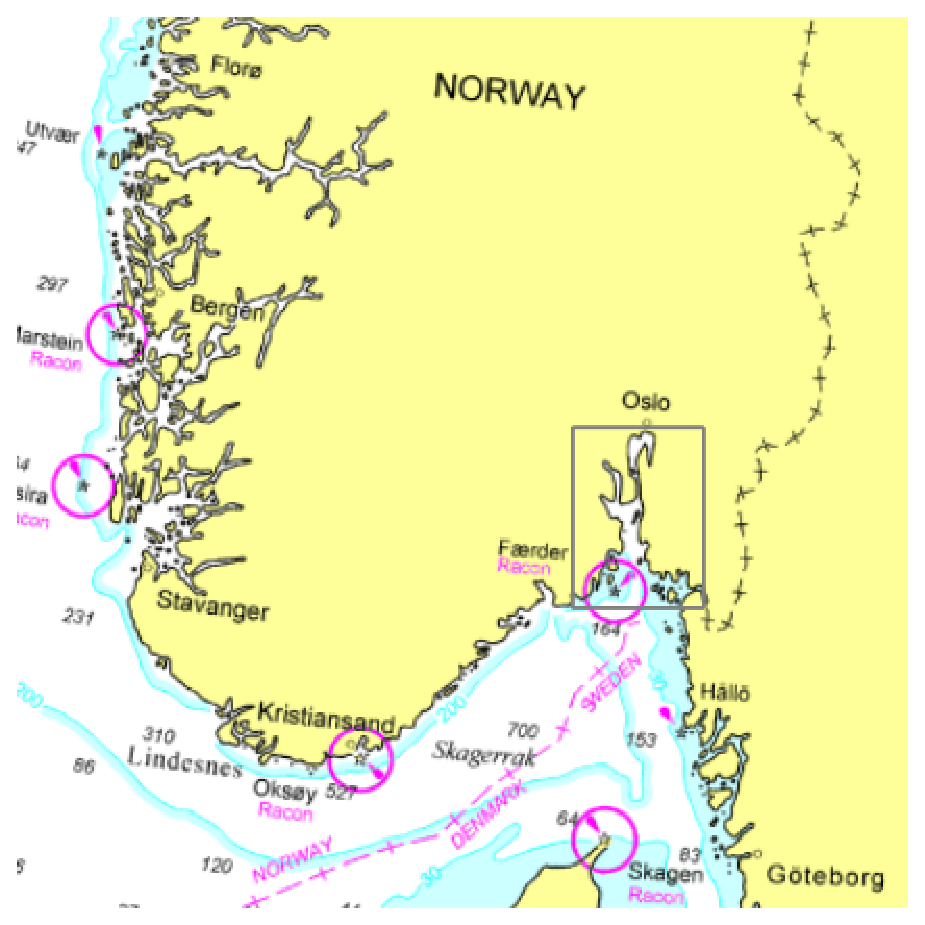
\includegraphics[height=7.3cm]{Map_location_Oslofjord_2}}
   \rput[br](15.0,0.0){\includegraphics[height=9cm]{dyp_old}}
   \psline[linewidth=0.5mm,linecolor=blue]{->}(13.4,5.3)(11.3,6.3)
   \psline[linewidth=0.2mm](4.45,4.95)(7.5,8.5)
   \psline[linewidth=0.2mm](4.45,3.5)(7.5,1)
  \end{pspicture}
% Figure caption is below the figure
  \caption{\small The topography and irregular coastline of the Oslofjord and its location in Southern Norway. The right-hand gray scale bar indicates depth in meters. The blue arrow points to the location of the fjord's main sill (the {\DR} sill as enlarged in Figure \ref{fig:droebak_sill}) which is only $\sim$ 20 m deep. Note also the $\sim$ 400 m deep basin extending from the Skagerrak towards the Hvaler Archipelago in the southeast, the so called Hvalerdjupet. }
  \label{fig:map_oslofj}       % Give a unique label
 \end{center}
\end{figure}
%


The {\DR} Sill is partly man made\footnote{The jetty was built in the years 1874 - 1879 as a naval defense of Oslo, the capital of Norway. It forces large vessels to sail east of the fortress Oscarsborg built at Kaholmen.} and partly natural. The natural sill is about 20 m deep, while the man made part is only 1-2 m deep. The latter consists of an underwater barrier, the {\DR} Jetty, extending halfway across the {\DR} Sound from the western mainland south of {\DR} to south of the small island Kaholmen located slightly to the east of the southern tip of the {\HAA} (Figure \ref{fig:droebak_sill}). There are two narrow openings in the Jetty with a maximum depth of about 6 m. One is located close to the mainland on the western side, while the second runs east-west and is located just south of Kaholmen.   
%%%%%%%%%%%%%%%%%%% Figure 2 Bathymetry and currents in the Drøbak area %%%%%%%%%%%%%%%
\begin{figure}[t]
 \begin{center}
  \begin{pspicture}(0,0)(15,9.2)
% Include graphs
   \rput[b](7.5,-0.8){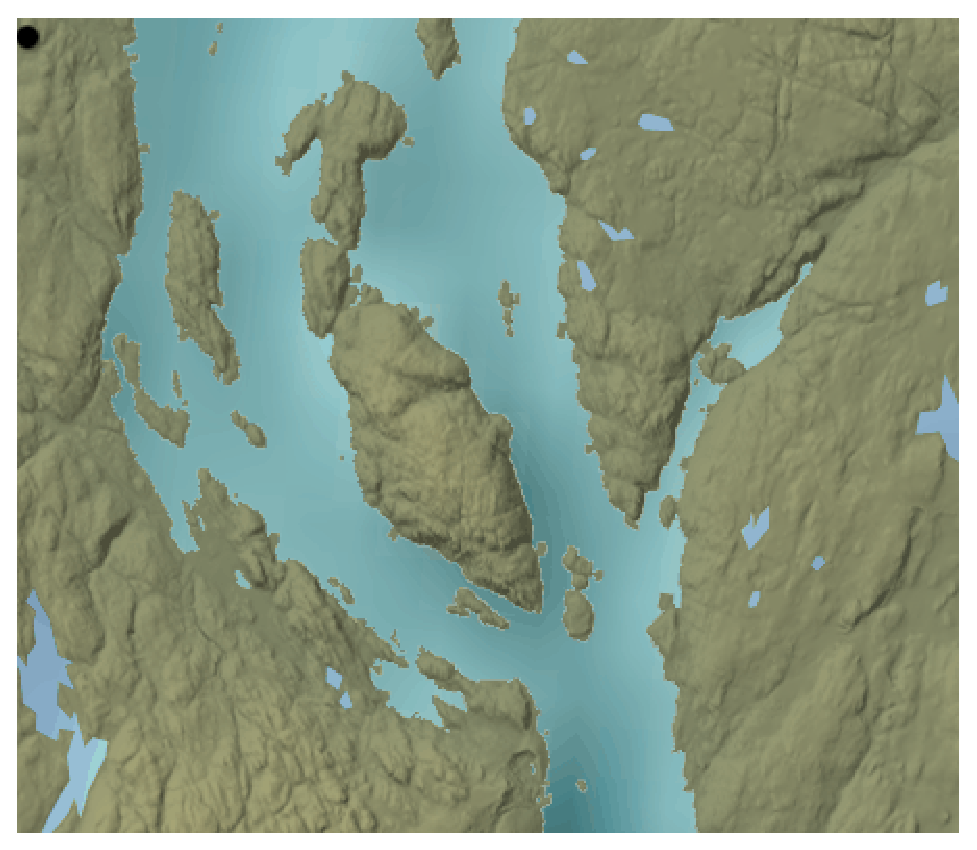
\includegraphics[height=10cm]{dyp_Drobak}}
  \end{pspicture}
  \caption{\small The irregular coastline and topography in the {\DR} Sill area.}
  \label{fig:droebak_sill}
 \end{center}
\end{figure}

 

The sill area represent a major obstruction for the water exchange between the inner and the outer part of the fjord. Due its narrowness and shallowness the {\DR} Sill area is famous for its strong tidal currents that can be as swift as 1 m/s. We also note that north of the sill the fjord is separated by {\HAA} into an eastern and a western channel each about 1 km wide. These channels and the openings in the Jetty are important to include in any model of the Oslofjord to obtain realistic circulation patterns and strengths in the area. Another noteworthy topographic feature is the Hvalerdjup located at the entrance to the fjord (Figures \ref{fig:map_oslofj} and \ref{fig:ferder_hvaler}). It is a 400 m deep basin extending northeastward from the Skagerrak towards the Hvaler Archipelago. As revealed by Figure \ref{fig:map_oslofj} there are also several other somewhat shallower basins $\sim$ 150 - 200 m deep as we proceed into the fjord. 
%%%%%%%%%%%%%%%%%%% Figure 2 Bathymetry and currents in the Drøbak area %%%%%%%%%%%%%%%
\begin{figure}[t]
 \begin{center}
  \begin{pspicture}(0,0)(15,8.8)
% Include graphs
   \rput[bl](-0.1,0){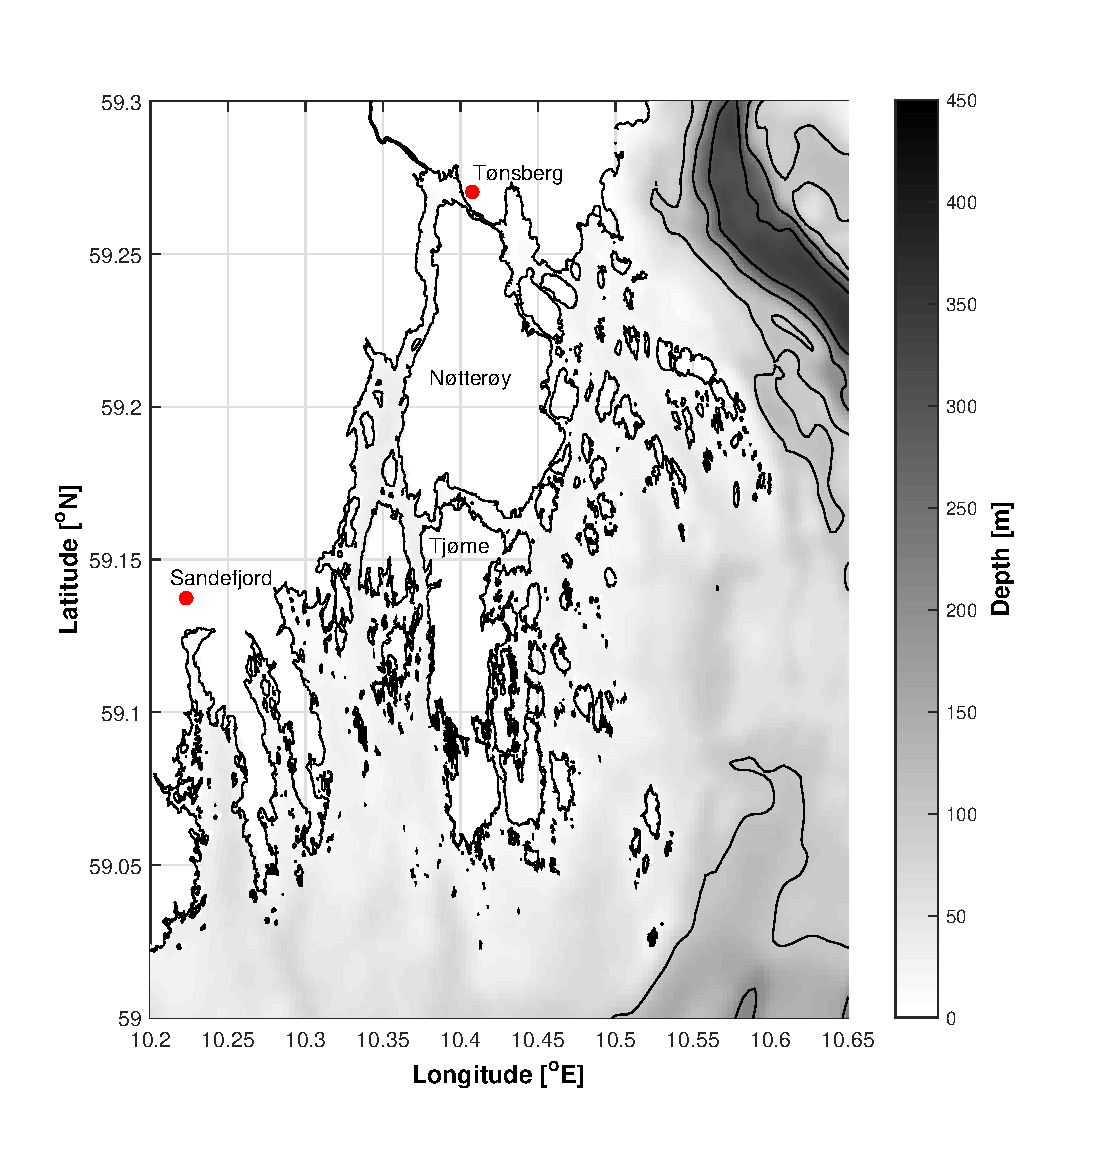
\includegraphics[height=8.8cm]{dyp_Tonsberg_old}}
   \rput[br](16.0,0){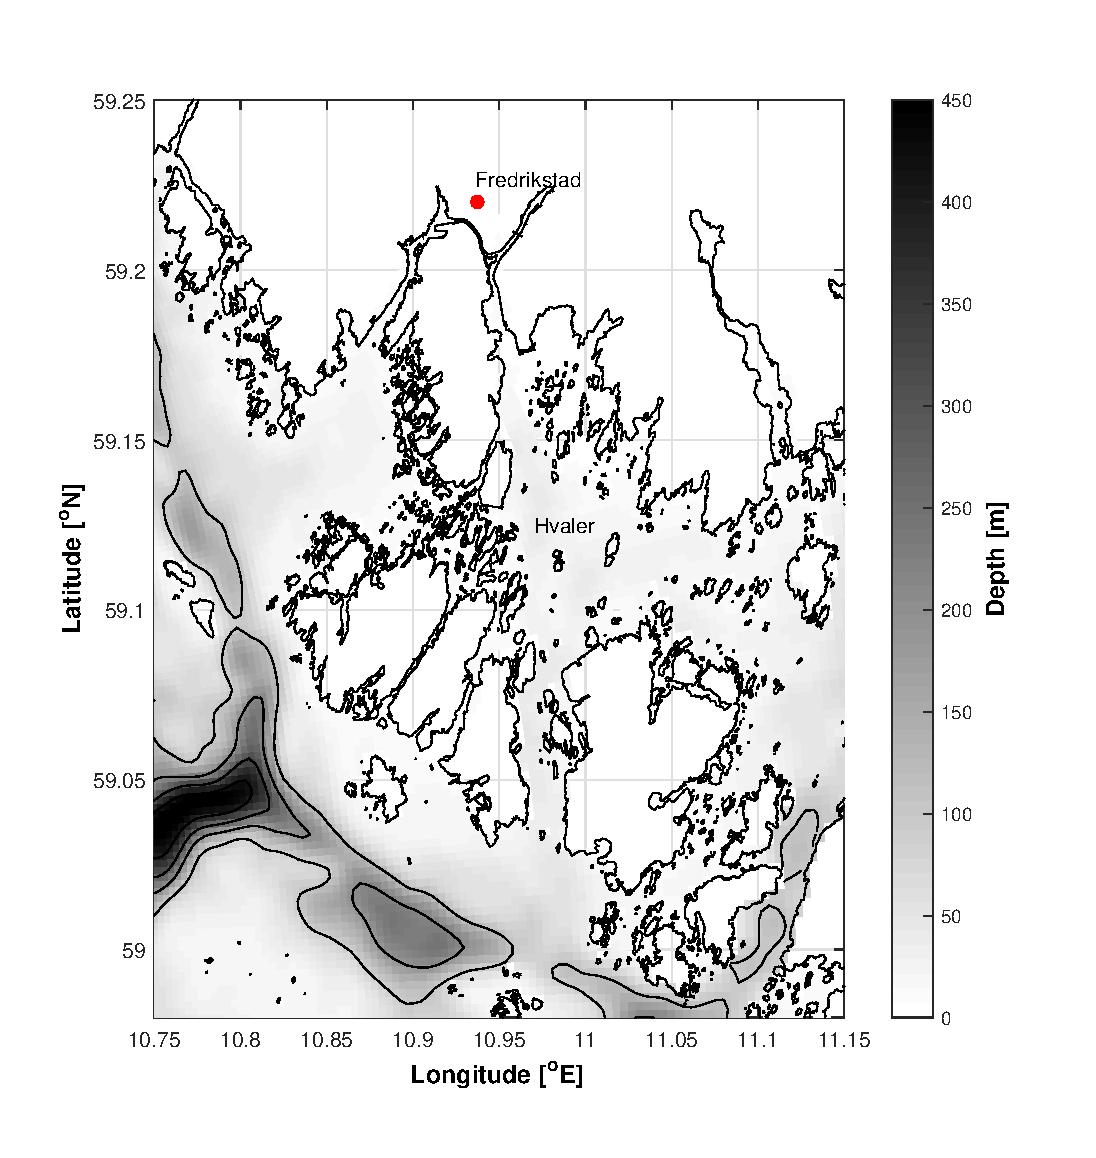
\includegraphics[height=8.8cm]{dyp_Hvaler_old}}
  \end{pspicture}
  \caption{\small The irregular coastline geometry and topography in the F{\ae}rder National Park (left-hand panel) and the Hvaler National Park (right-hand panel). Note the many islands, narrow straits and channels present in these areas of the Oslofjord.}
  \label{fig:ferder_hvaler}
 \end{center}
\end{figure}

 

In addition to the {\DR} Sill area there are other areas in the fjord that features many smaller and larger islands. For instance to the west we find the T{\o}nsberg Archipelago including Bol{\ae}rne, Store and Lille F{\ae}rder (F{\ae}rder Lighthouse), and to the east we find Rau{\o}y and Hank{\o} including the smaller Island S{\o}strene and Misingene and the Hvaler Archipelago (Figure \ref{fig:ferder_hvaler}). Further north on the west side of the fjord we find Bast{\o} south of Horten, and to the east Jel{\o}ya just west of Moss. Jel{\o}ya is separated from the mainland by a narrow channel about 50 m wide within which water sloshes back and forth with the tides \citep{hjelm:etal:2014}. The presence of these archipelagos with its small islands give rise to many narrow sounds, straits and channels impeding the water exchange. If the goal is to compute realistic pathways of any unwanted substances discharged to the fjord or trajectories of floating structures including man overboard (Search and Rescue Services), we need to resolve, to the best of our ability, these features. 

Finally it is worth mentioning the many rivers discharge freshwater to the fjord. For instance two of Norway's largest rivers, namely Glomma and Drammenselva\footnote{Here it is chosen to use Norwegian river names in which ``elv'' or ``vassdrag'', means ``river'' or ``water course''.}, are emptying their freshwater into the Oslofjord with a mean discharge of 729 and 317 m$^3$/s, respectively \citep{milli:etal:2011}. This freshwater has a decisive impact on the salinity and hence on the circulation in the fjord. Furthermore, in most fjords the river outlet is located at the fjord head leading to an estuarine circulation. In contrast the Glomma outlet is located in the outer part of the Oslofjord within the Hvaler Archipelago, while the Drammenselva outlet is located in the middle part of the fjord. As a result the estuarine circulation in the Oslofjord deviates considerably from a classical textbook example.        
%%%%%%%%%%%%%%%%%%%%%%%%%%% Figure 3 Godafoss %%%%%%%%%%%%%%%%%%%%%%%%%%%%%%%
\begin{figure}[t]
 \begin{center}
  \begin{pspicture}(0,0)(15,5.5)
% Include graphs
   \rput[bl](0.0, 0.0){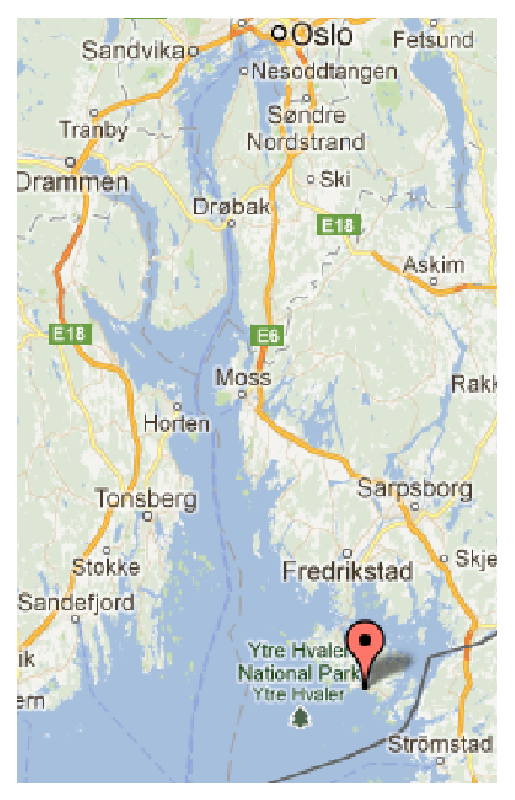
\includegraphics[height=5.5cm]{Fig03}}
   \rput[br](15.0,0.0){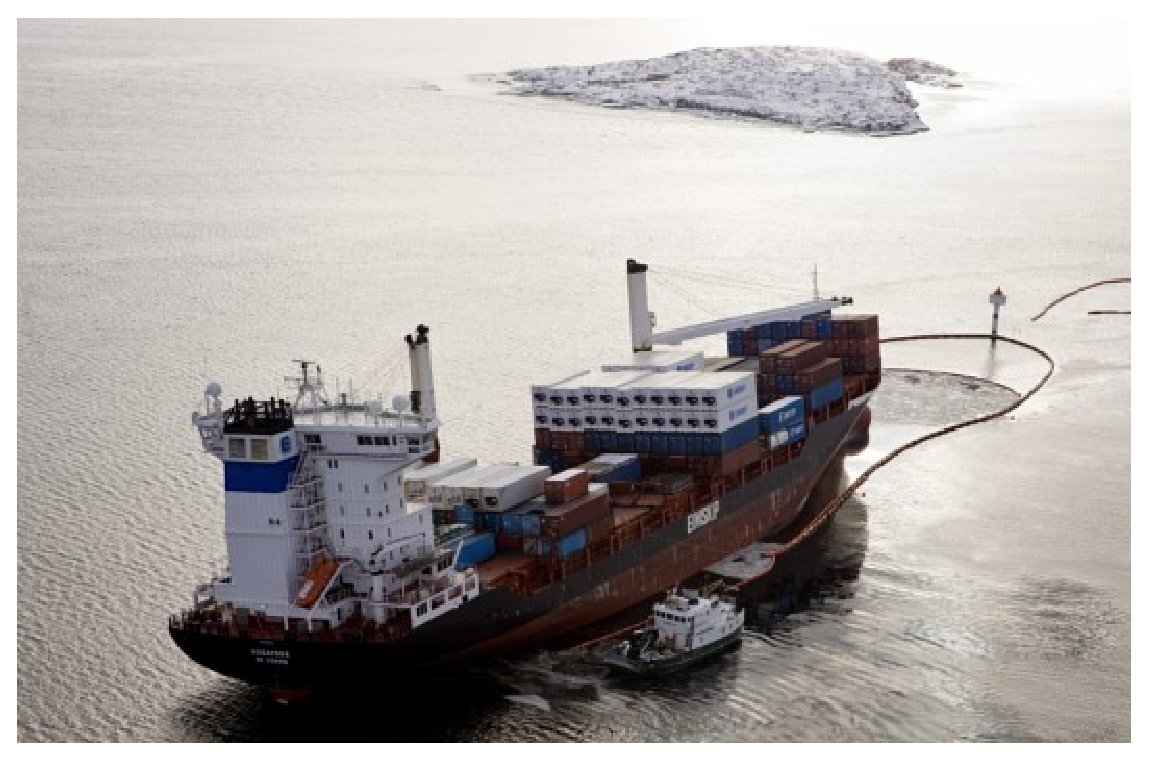
\includegraphics[height=5.5cm]{Fig03_2}}
  \end{pspicture}
  \caption{\small Map (left) showing the location where the ship ``Godafoss'' (right) grounded February 17, 2011. The location is in the sound L{\o}peren between two of the major islands in the Hvaler Archipelago where Norway's largest river flows through on its way to the Oslofjord.} 
  \label{fig:godafoss}
 \end{center}
\end{figure}



% % % % % % % % % % % % % % % % % % % % % % % % % % % % % % % % 
\subsection{Why a new model?}
The Oslofjord is somewhat special among the Norwegian fjords from a physical as well as a societal perspective. The population surrounding it, or more precisely people living less than one hours drive from the Oslofjord, comprises 40\% of the Norwegian population according to the official statistics\footnote{\texttt{http://www.ssb.no} as of July 1, 2012}. This is by far the most populated area in Norway, a population that is steadily growing. Moreover, no other fjord has anything close to as high density of leisure boats. In addition the Oslofjord features two of Norway's national underwater parks, the Hvaler National Park\footnote{\texttt{http://www.ytrehvaler.no/}} and the F{\ae}rder National Park\footnote{\texttt{http://prosjekt.fylkesmannen.no/faerdernasjonalpark/Om-Farder-nasjonalpark/}}. Thus, taking into account that the Oslofjord has the largest traffic density of commercial vessels of all the Norwegian fjords the risk of an accident resulting in a possible, unwanted contaminated effluent to the fjord is uncomfortably high. 
%%%%%%%%%%%%%%%%%%%%%%%%%%% Figure 3 Godafoss %%%%%%%%%%%%%%%%%%%%%%%%%%%%%%%
\begin{figure}[t]
 \begin{center}
  \begin{pspicture}(0,0)(15,11)
% Include graphs
   \rput[b](7.7, 0.0){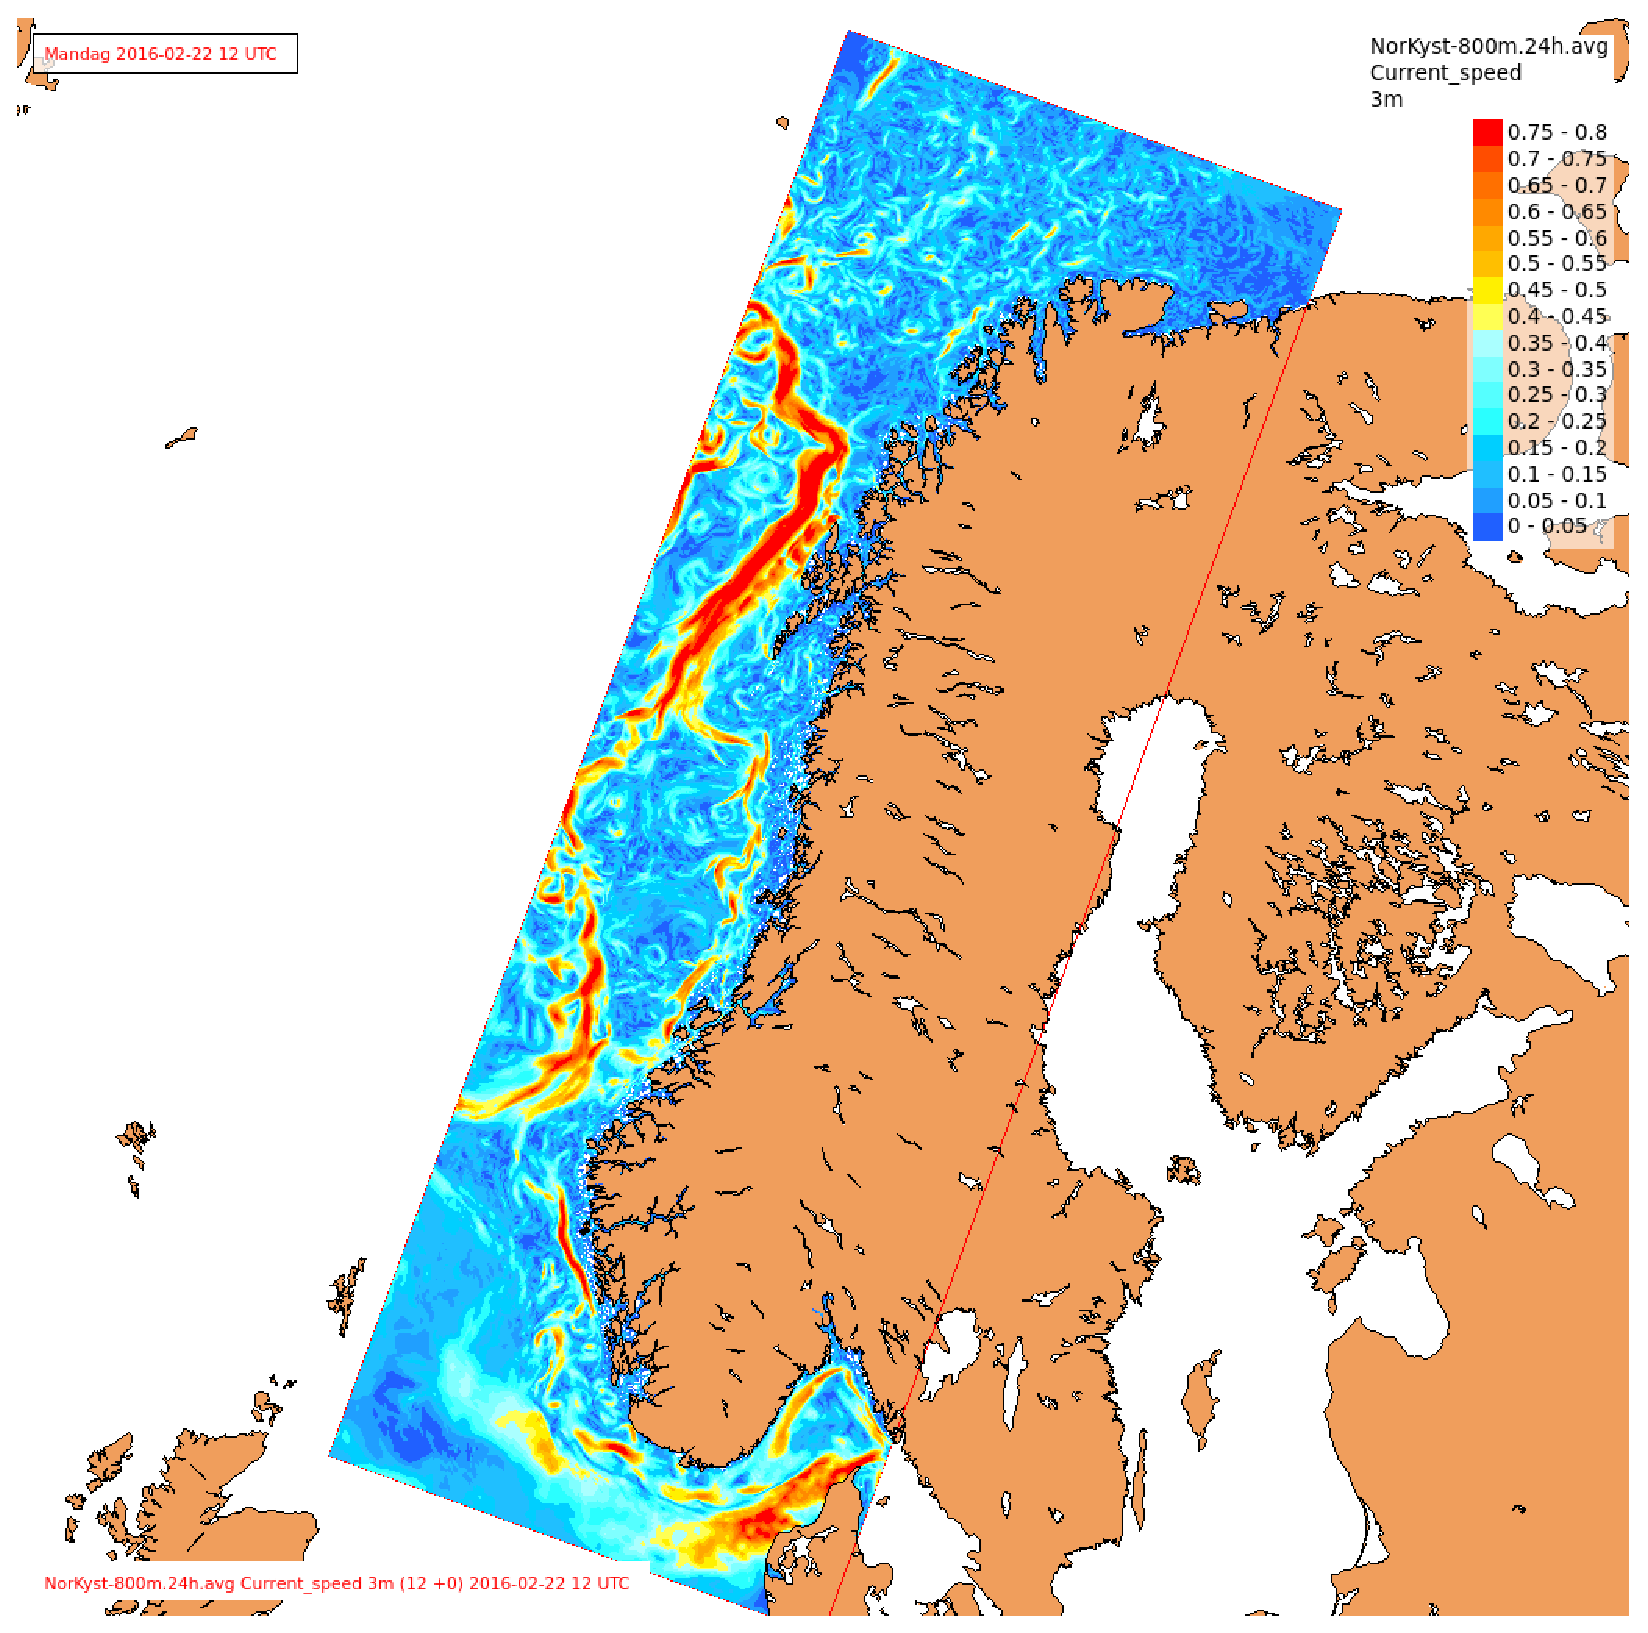
\includegraphics[height=11cm]{N800_2016-02-22_SPEED_3m_24h_avg}}
  \end{pspicture}
  \caption{\small The area covered by the NorKyst800 model. Shown is forecasted, 24 hour average speed at 3 m depth valid for February 22, 2016. Color bar gives speed in m/s with a a contour interval of 0.05 m/s.} 
  \label{fig:n800}
 \end{center}
\end{figure}

 

An example of such an unwanted event is the Godafoss accident. On February 17, 2011 the ship ``Godafoss'' grounded in a narrow sound in the Hvaler Archipelago (Figure \ref{fig:godafoss}). As a result a lot of its fuel oil was discharged into the fjord. When an event like this happens MET Norway has to, within half an hour, forecast the dispersion, drift and spreading of the oil as part of its emergency preparedness\footnote{On behalf of the Norwegian Coastal Administration (Kystverket)}. Recall that most of the accidents like Godafoss tend to happen within archipelagos\footnote{\texttt{https://en.wikipedia.org/wiki/List\_of\_oil\_spills}}. The safety of the people that utilize the fjord, and the protection of its environment, is therefore a challenge to governmental agencies, regional administrations and local management alike. 

One of the key inputs to the emergency preparedness models for oil drift is ocean currents and temperature together with wave and atmospheric input. The present model providing forecasts of ocean currents and temperature for the Oslofjord, and which is run operationally by MET Norway on a 24/7 basis, is the NorKyst800 model \citep{albre:etal:2011}. As depicted by Figure \ref{fig:n800} it covers not only the Oslofjord, but actually the entire Norwegian coast. It was developed to capture mesoscale phenomena such as jet currents, eddies and meanders in Norway's near coastal areas, and to provide forecasts of some reliability in the fjords. It was set-up with a regular grid of 800x800 m, a grid of high enough resolution to resolve the Rossby radius of deformation required to capture the mesoscale phenomena in Norway's near coastal waters. 
%%%%%%%%%%%%%%%%%%%%%%%%%%% Figure 3 Godafoss %%%%%%%%%%%%%%%%%%%%%%%%%%%%%%%
\begin{figure}[t]
 \begin{center}
  \begin{pspicture}(0,0)(15,5.2)
% Include graphs
   \rput[bl]( 0.0,0.0){
\includegraphics[height=5.2cm]{Oslofjord_A20_grid}}
   \rput[b ]( 7.5,0.0){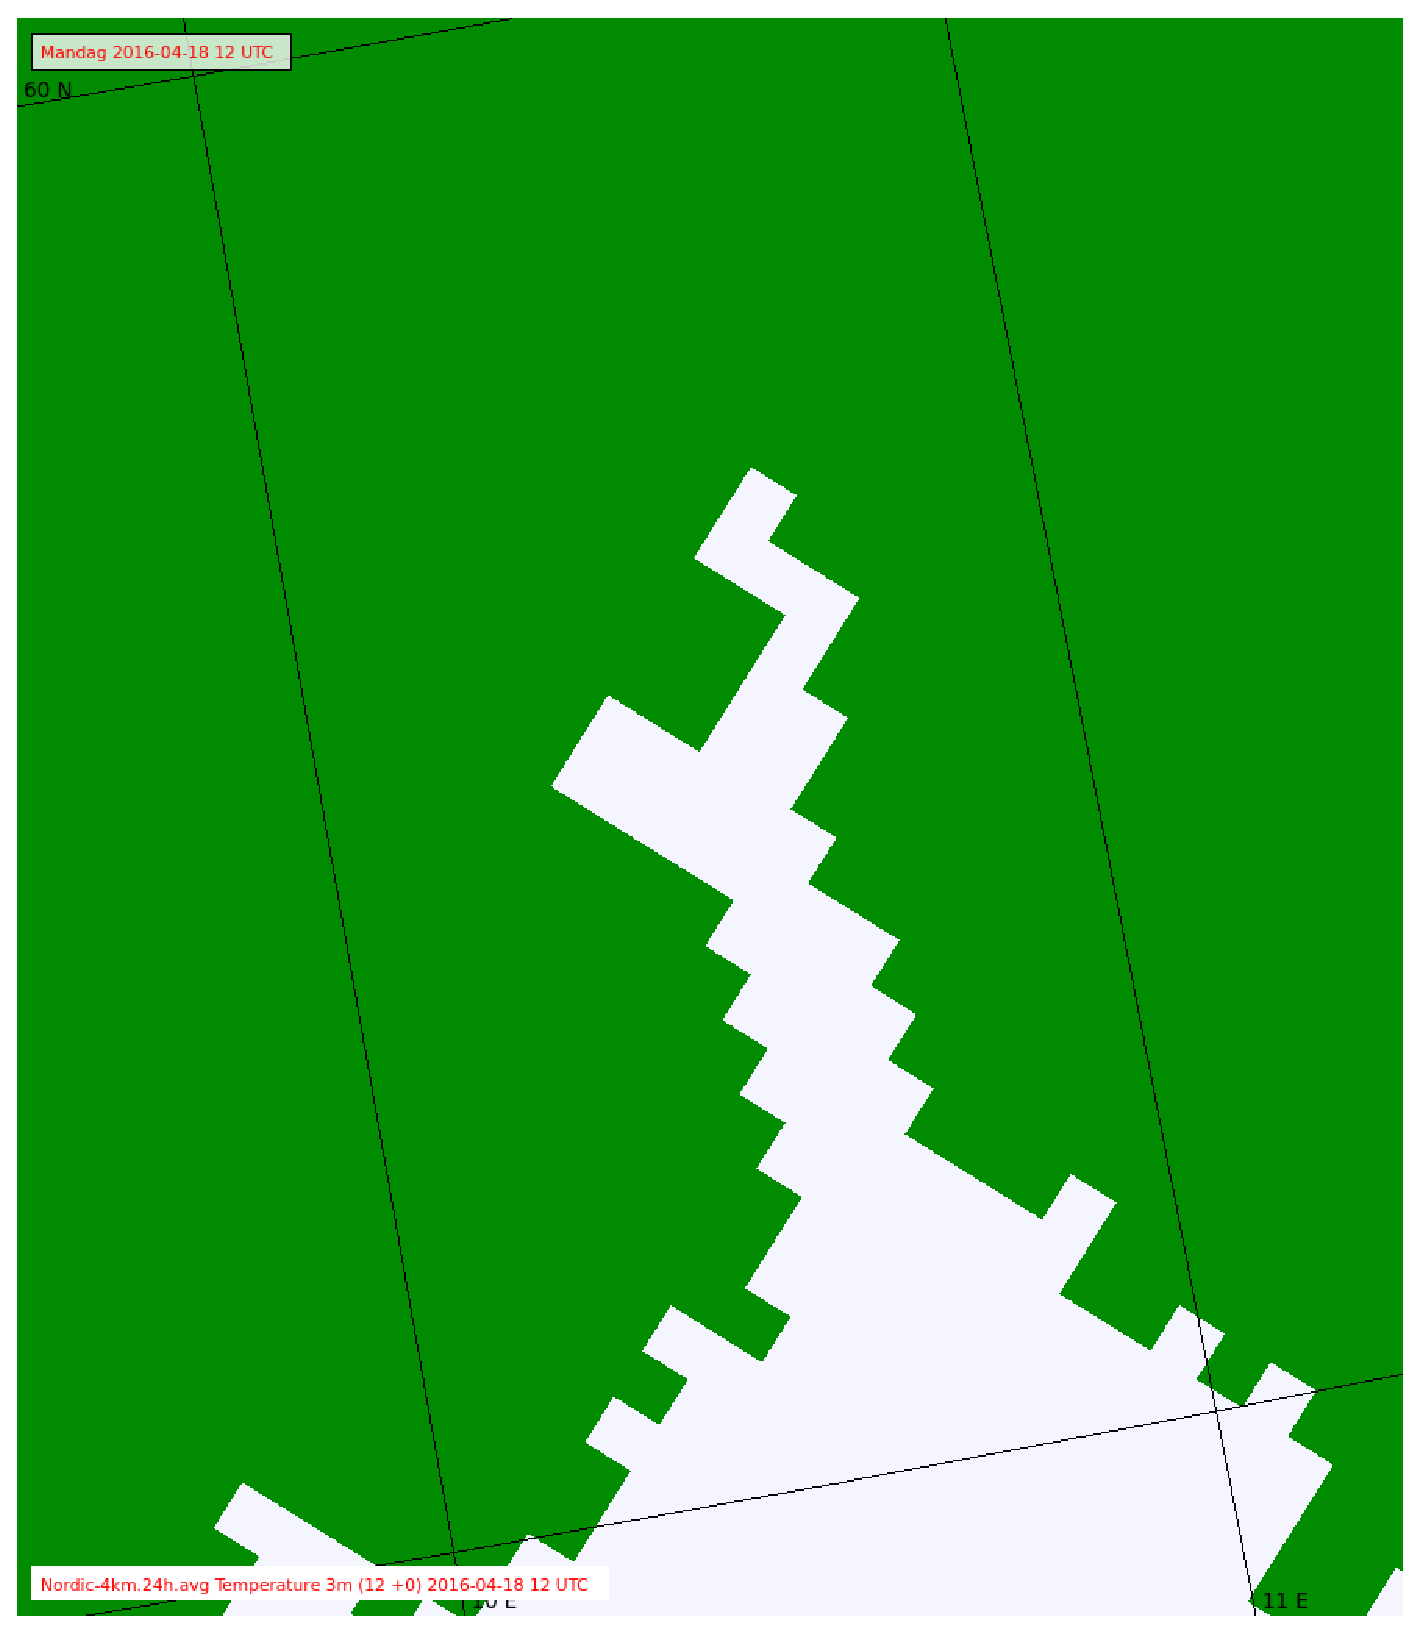
\includegraphics[height=5.2cm]{Oslofjord_N4_grid}}
   \rput[br](15.0,0.0){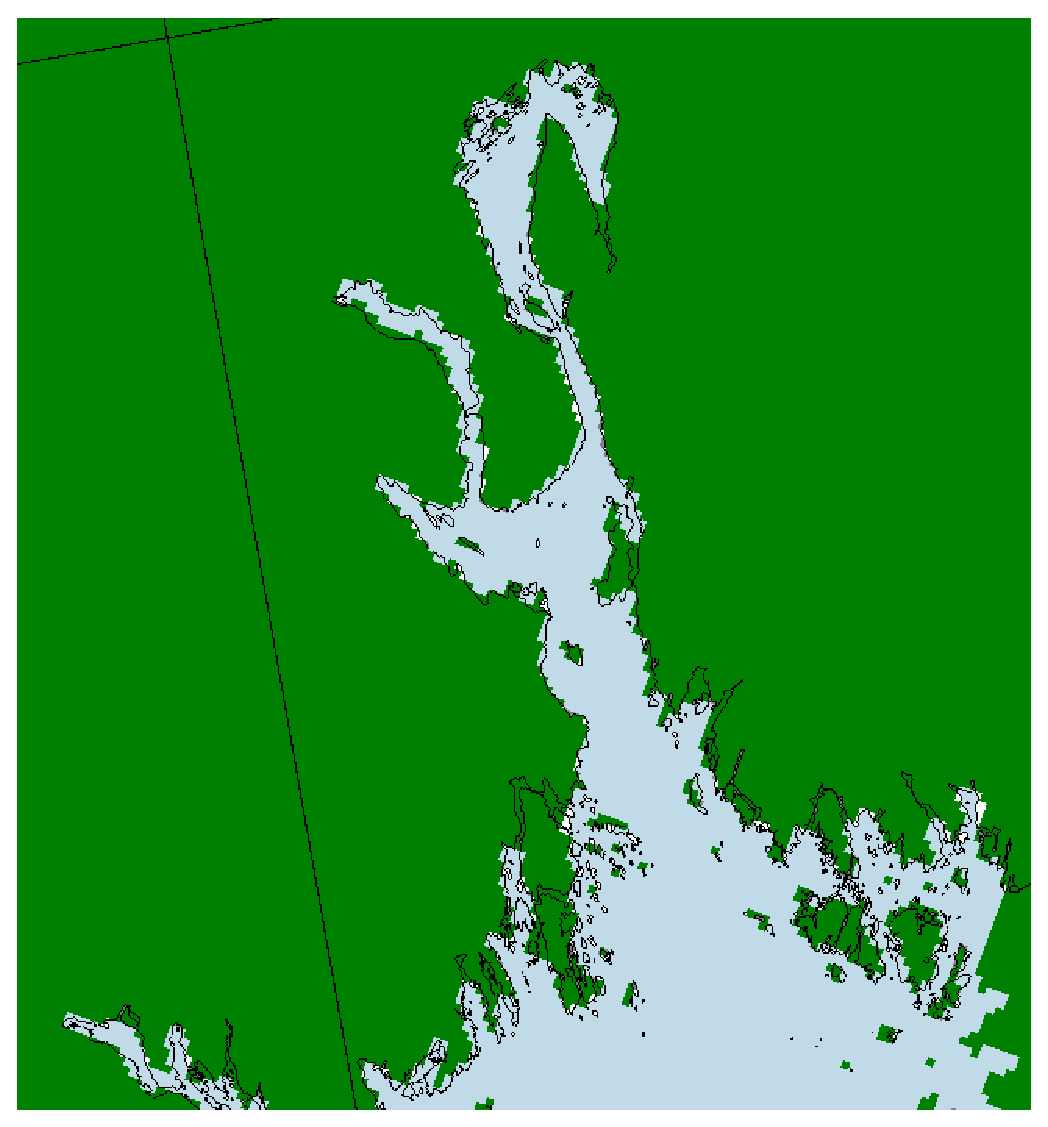
\includegraphics[height=5.2cm]{Oslofjord_N800_grid}}
   \rput[bl]( 0.3,4.7){\large \textbf{a)}}
   \rput[b ]( 5.6,4.7){\large \textbf{b)}}
   \rput[br](10.9,4.7){\large \textbf{c)}}
  \end{pspicture}
  \caption{\small Map of the Oslofjord overlayed by a 20 km grid size (a), 4 km grid size (b) and 800 m grid size (c) model.} 
  \label{fig:resolution}
 \end{center}
\end{figure}



Nevertheless the resolution offered by NorKyst800 is not fine enough to resolve the highly irregular geometry and topography of most Norwegian fjords, and the Oslofjord is no exception. These irregularities consist of small islands, narrow sounds, straits and channels and many smaller scale deep basins and shallow sills (Figure \ref{fig:map_oslofj}). To properly be prepared to forecast the transport and spreading of any unwanted substances or contaminants accidentally discharged to the fjord it is of importance that the underlying fjord model resolves the \emph{sub}mesocale phenomena generated by the presence of these irregularities, in addition to resolve the mesoscale phenomena. We emphasize that such a model, when operational, will benefit all emergency preparedness models that is operated by MET Norway. Examples of such models are, in addition to oil drift, (i) Search And Rescue (SAR) which involves forecasting of pathways of floating objects such as man overboard, rafts, small crafts and ships, (ii) transport and spreading of dissolved substances such as nutrients, nuclear waste and other dissolved toxic substances, and (iii) growth and drift of toxic algae. Finally we emphasize that resolving the submesoscale motion due to the fjord's irregular geometry and topography is required to avoid floating objects, dissolved substances and oil from stranding artificially.  

How the resolution impacts on how well the model portrays these irregularities is perhaps best illustrates by Figures \ref{fig:resolution} and \ref{fig:resolution_2}. The former shows how the Oslofjord is depicted in, respectively, a 20 km, 4 km and 800 m grid, while the latter, focusing on an enlargement of the area between {\DR} and T{\o}nsberg, depicts how the fjord is portrayed in, respectively, a 4 km, 800 m and 100 m grid. As is evident from Figure \ref{fig:resolution} it is only the 100 m grid that represents the fjord as something that looks like the Oslofjord geometry as we know it from geographical charts and maps. Zooming in on Breidangen (Figure \ref{fig:resolution_2}) we observe that it takes at least a 100 m grid to properly represent the many narrow straits, channels and islands present in the fjord. For instance we note the presence of small islands in Breidangen present in the 100 m grid which is simply not there in the 800 m grid. Likewise the shape and area covered by Bast{\o}y is improved in the 100 m grid, and so is the ridge that cuts into the the Drammensfjord at Svelvik. The same is true regarding topography as displayed in Figure \ref{fig:hvaler2} comparing the Hvalerdjupet in the NorKyst800 model with the 100 m resolution topography. 
%%%%%%%%%%%%%%%%%%%%%%%%%%% Figure 3 Godafoss %%%%%%%%%%%%%%%%%%%%%%%%%%%%%%%
\begin{figure}[t]
 \begin{center}
  \begin{pspicture}(0,0)(15,6.5)
% Include graphs
   \rput[bl]( 0.0,0.0){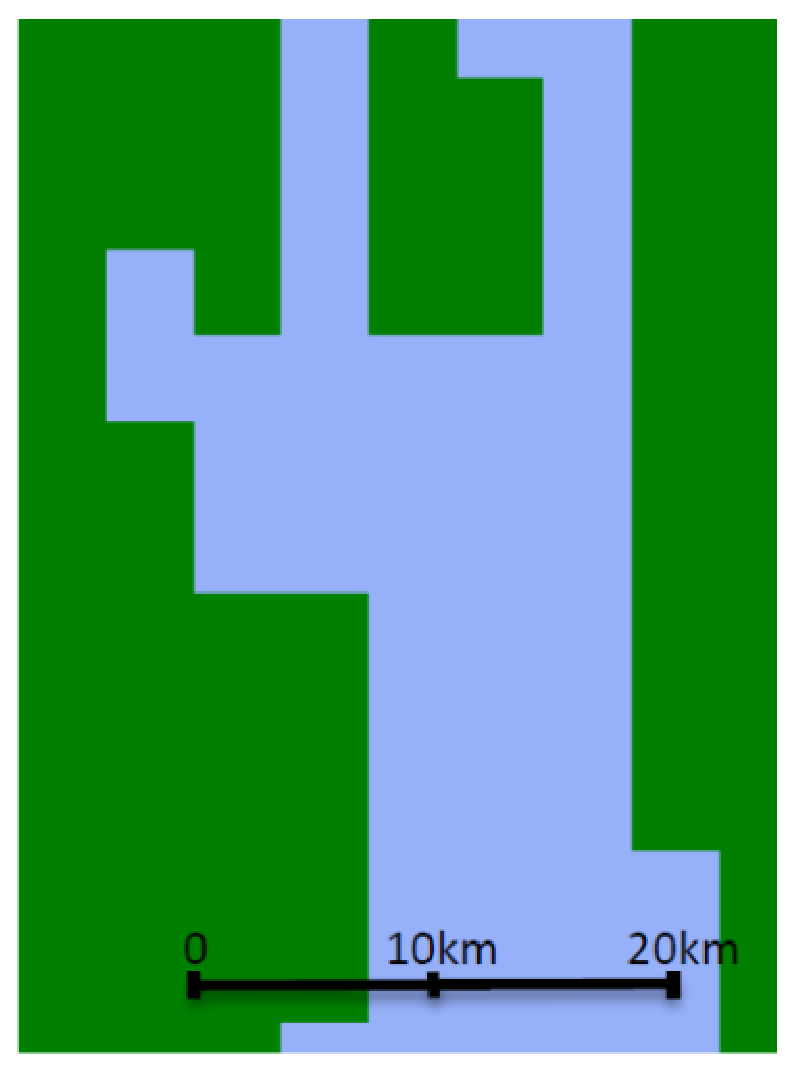
\includegraphics[height=6.5cm]{Midfjord_N4_grid}}
   \rput[b ]( 7.5,0.0){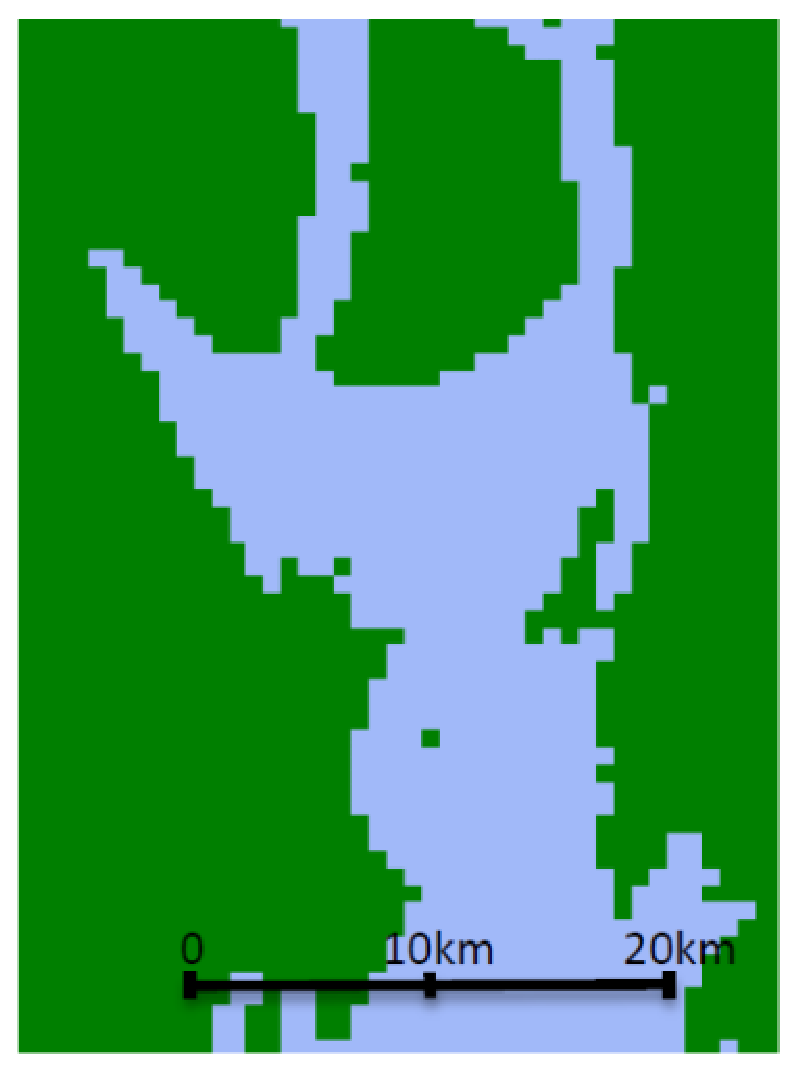
\includegraphics[height=6.5cm]{Midfjord_N800_grid}}
   \rput[br](15.0,0.0){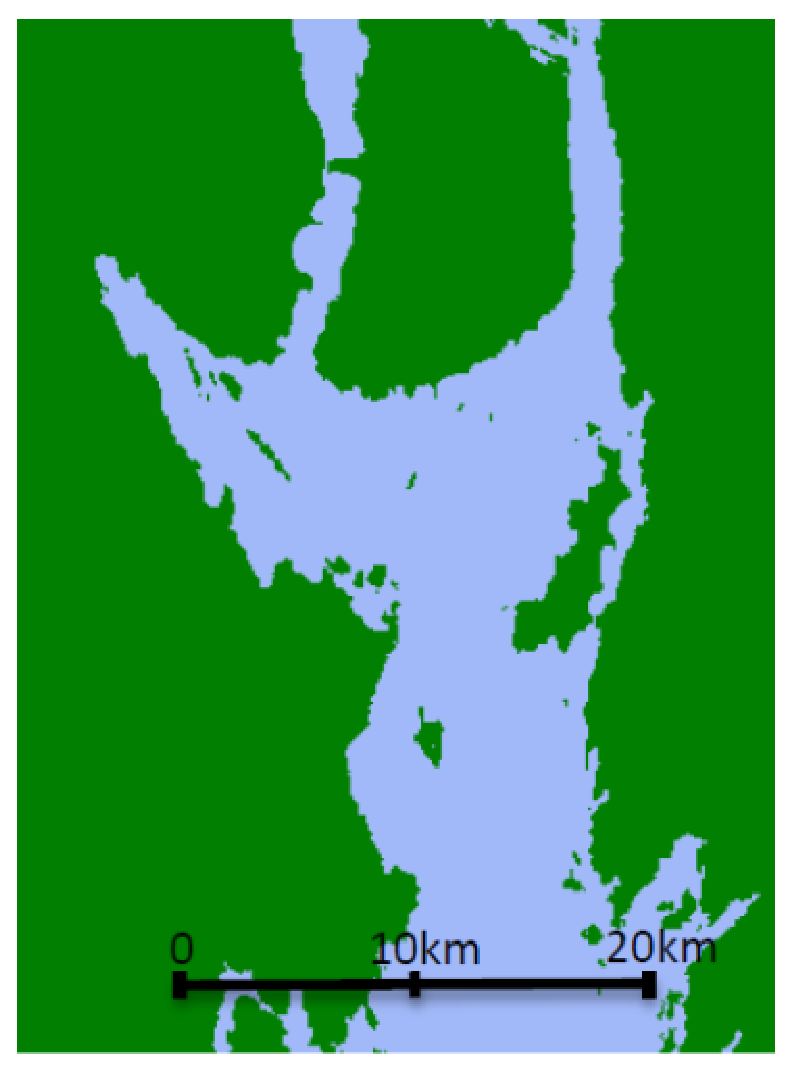
\includegraphics[height=6.5cm]{Midfjord_100m_grid}}
   \rput[bl]( 0.3,6.0){\large \textbf{a)}}
   \rput[b ]( 5.6,6.0){\large \textbf{b)}}
   \rput[br](10.9,6.0){\large \textbf{c)}}
  \end{pspicture}
  \caption{\small As Figure \ref{fig:resolution}, but zoomed in on Breidangen. To better reveal the grid the underlying map is not shown. (a) 4 km grid, (b) 800 m grid and (c) 100 m grid. Note that it takes a 100 m grid to properly resolve the many islands, narrow straits and channels present in the fjord. } 
  \label{fig:resolution_2}
 \end{center}
\end{figure}



To conclude the present forecasting models for the Oslofjord (NorKyst800) has an insufficient resolution, and a new model of the Oslofjord with a resolution of 100 m or less, at least in parts of the fjord, is in need. The development of a such a model would also greatly benefit the other emergency preparedness products delivered by MET Norway on behalf of other governmental institutions and agencies, e.g., the Norwegian Coastal Administration (Kystverket) and the Norwegian Radiation Protection Authorities (NRPA).   
%%%%%%%%%%%%%%%%%%% Figure 2 Bathymetry and currents in the Drøbak area %%%%%%%%%%%%%%%
\begin{figure}[t]
 \begin{center}
  \begin{pspicture}(0,0)(15,8.5)
% Include graphs
   \rput[tl](-0.1,9.5){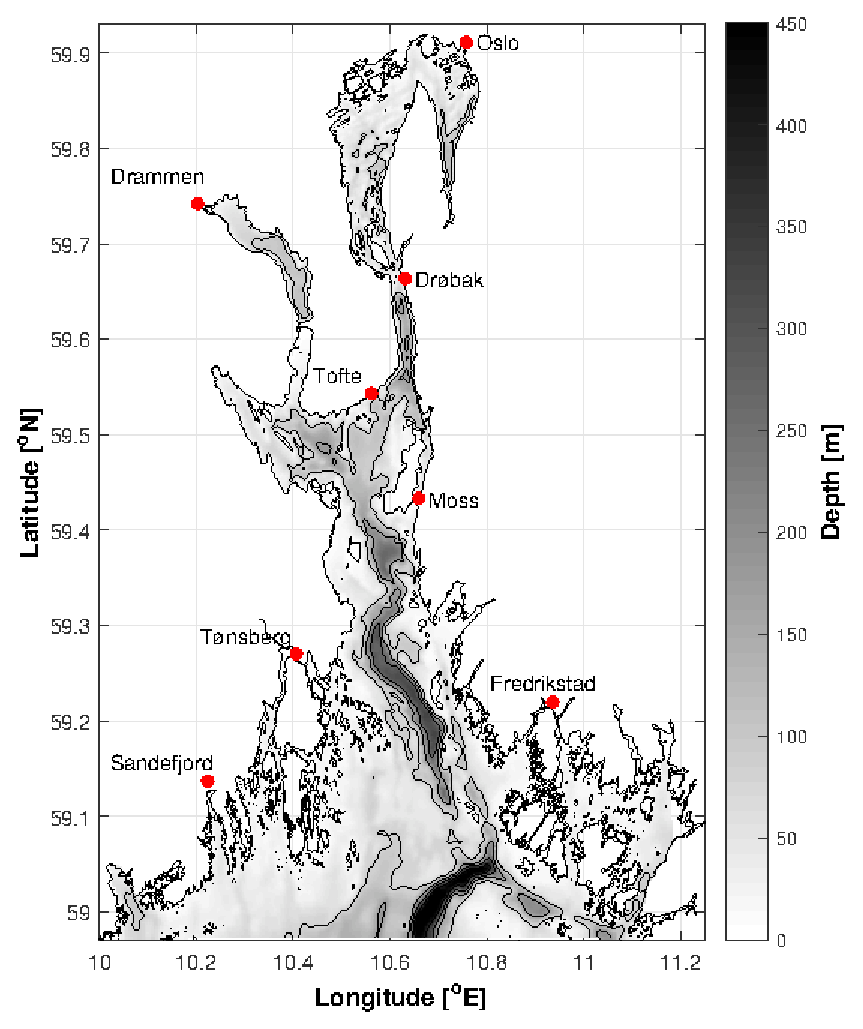
\includegraphics[height=8.5cm]{dyp}}
   \rput[tr](  15,9.5){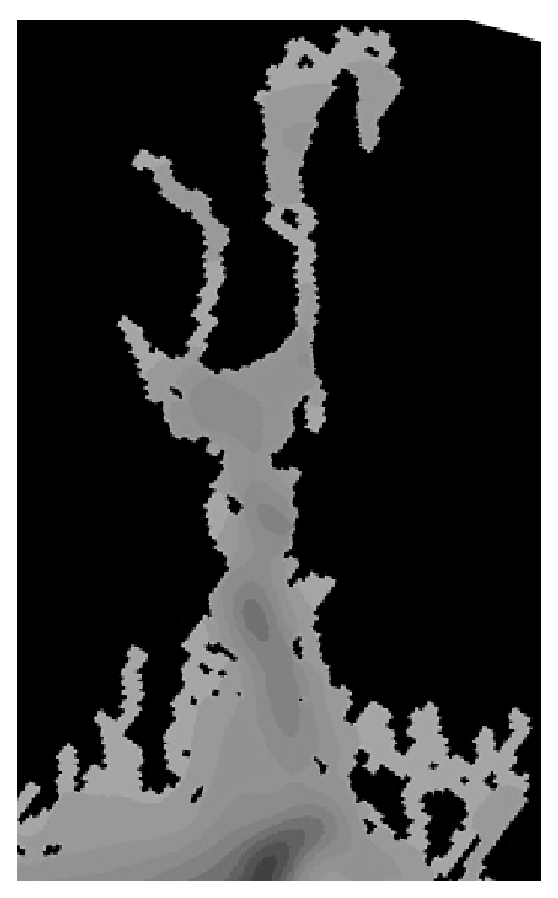
\includegraphics[height=8.0cm]{NorKyst800_topo_oslofjord}}
  \end{pspicture}
  \caption{\small The irregular coastline geometry and topography in the Oslofjord as portrayed in the FjordOs CL model (left) and the NorKyst800 model (right). The color bar (grayscale) indicate depth in meters.}
  \label{fig:hvaler2}
 \end{center}
\end{figure}



% % % % % % % % % % % % % % % % % % % % % % % % % % % % % % % % 
\subsection{Organization of the report}
The report is organized as follows. Section \ref{sec:model} provides some details on how the curvilinear grid of the FjordOs CL model is constructed. Section \ref{sec:setup} provides some model specifics while Section \ref{sec:forcing} gives details on the model's bathymetry and external forcing such as tides, ocean input through open lateral boundaries, river input as well as atmospheric input. Section \ref{sec:resul} provides some results from an almost two year long hindcast and some test forecasts. Finally we offer a summary and some concluding remarks in Section \ref{sec:summa}. 


%%%%%%%%%%%%%%%%%%%%%% The triply nested grid configuration %%%%%%%%%%
\section{The new model}
\label{sec:model}
The FjordOs CL model is based on version 3.6 of the Rutgers Regional Ocean Modeling System (ROMS) adapted to the Oslofjord. ROMS is an open source, numerical ocean model as detailed and documented by \cite{haidv:etal:2008}, \cite{shche:mcwil:2003} and \cite{shche:mcwil:2005, shche:mcwil:2009}. It is freely available and may be downloaded from the ROMS website\footnote{\texttt{http://www.myroms.org/}}. 

In summary ROMS is a free-surface and terrain-following, vertical coordinate ocean model, based on the fully three-dimensional, rotational RANS\footnote{Reynolds Average Navier-Stokes} equations utilizing the hydrostatic and Boussinesq approximations. It is a so called split–explicit model where short time steps are used to advance the surface elevation and barotropic momentum equation, and where a much larger time step is used for temperature, salinity, and baroclinic momentum. In this ROMS employs a two-way time-averaging procedure for the barotropic mode which satisfies the 3D continuity equation. 

% % % % % % % % % % % % % % % % % % % % % % % % % % % % % % % % 
\subsection{Why ROMS?}
An option in ROMS is to use a curvilinear, near orthogonal grid to replace the default orthogonal regular mesh. This option is exploited here. The rationale is that it allows us to minimize the number of, or in reality the area of, ``dry'' grid points. Thereby the number of ``wet'' grid points is maximized without increasing the number of grid points compared to an orthogonal, regular grid mesh model covering the same domain. Thus resolution is increased without increasing the computational burden. In addition it allows us, to a certain extent, to put higher resolution in areas of special interest.

The above may also be achieved using unstructured grid models (e.g., FVCOM\footnote{\texttt{http://fvcom.smast.umassd.edu/fvcom/}}, SLIM\footnote{\texttt{http://sites.uclouvain.be/slim/}}). However, the FjordOs research group opted to go for a ROMS development utilizing its curvilinear option rather than starting a completely new strand of model development. The rationale is that 1) ROMS is MET Norway's operational model, 2) MET Norway's scientists are well versed in using ROMS, and 3) MET Norway's scientists have the necessary expertise to operate it. Moreover, none of researchers within the FjordOs participating institutions have any beforehand experience in running and/or setting up a three-dimensional, unstructured model. Nevertheless, to get some insight into the capabilities of an unstructured model, a \emph{two-dimensional version} of FVCOM was used as part of the FjordOs project for the work regarding Moss Harbor \citep{hjelm:etal:2014}.  
%%%%%%%%%%%%%%%%%%%%%%%%%%% Figure 9 FjordOs sketch %%%%%%%%%%%%%%%%%%%%
\begin{figure}[t]
 \begin{center}
  \begin{pspicture}(0,0)(15,10)
   \rput[bl](-0.2,0.0){\includegraphics[height=9.0cm]{fig4_crop}}
   \rput[br](15.0,0.0){\includegraphics[height=9.0cm]{res_crop}}
   \rput[bl]( 5.0,5.0){\textbf{a)}}
   \rput[br](13.0,5.0){\textbf{b)}}
  \end{pspicture}
  \caption{\small The FjordOs CL computational domain showing (a) the curvilinear grid configuration, and (b) the resulting grid resolution. The right-hand color bar indicates grid size in meters, while the left-hand bluescaled colorbar indicates depth in meters. X-axis is degrees east, and y-axis is degrees north.} 
  \label{fig:fjordos_grid}
 \end{center}
\end{figure}

   

% % % % % % % % % % % % % % % % % % % % % % % % % % % % % % % % 
\subsection{The curvilinear FjordOs CL grid}
Our implementation is inspired in parts by models like the ChesROMS\footnote{\texttt{http://ches.communitymodeling.org/models/ChesROMS/}} model that applied the curvilinear option for an implementation of ROMS for Chesapeake Bay. There exists several different software packages (MATLAB, Fortran, Python, etc.) that can be used for creating curvilinear grids with variable horizontal resolution for ROMS. We use the python-based software package OCTANT\footnote{\texttt{https://github.com/hetland/octant}}. The outer borders of the model domain is defined by corners and nodes as depicted in Figure \ref{fig:fjordos_grid} where corners are depicted as triangles and the nodes as circular dots. There should be a total of exactly four corners to limit the domain. ``Bends'' or nodes in the side walls are then specified so as to follow the land-sea matrix. For this first version of the FjordOs model, we have chosen the corners and nodes using a ``trial-and-error'' approach, so the geometry might be changed in future versions of the FjordOs CL model.

When creating the grid the main constraint is that the grid should be as close to being orthogonal as possible in particular at wet points. One of the advantages of using a package, as for instant the OCTANT package, is that it automatically achieves an optimal orthogonality. To help OCTANT achieving this we have kept the corners and nodes at dry points. The resulting model grid consists of 300 x 900 grid points in the horizontal. As shown by Figure \ref{fig:fjordos_grid} the grid size is less than 200 m in most of the wet areas of the fjord, and less than 100 m in most areas north of Slagentangen (at 59.3N). The exceptions are locations along and close to the southern border where the fjord widens and borders on Skagerrak. Here the grid size of the wet points varies from 200 to 350 m. The increased resolution is perhaps best visualized by Figure \ref{fig:fjordos_cl} displaying the Oslofjord in the curvilinear grid coordinates. Recall that in this coordinate system the grid points are equally spaced. Thus Breidangen and the inner Oslofjord is stretched out in the east-west direction. In reality Breidangen is about one third of the geographical distance across the southern open boundary. Thus the resolution in Breidangen and the inner Oslofjord is in effect increased with a factor of three. In the {\DR} sound the east-west grid size in the curvilinear grid is about 80 m.  
%%%%%%%%%%%%%%%%%%%%%%%%%%% Figure 8 FjordOs ROMS %%%%%%%%%%%%%%%%%%%%
\begin{figure}[t]
 \begin{center}
  \begin{pspicture}(0,0)(15,10)
%  \begin{pspicture}(0,0)(15,18.5)
% Include graphs (the ratio of height to width must be 18.5/8)
% Stående
   \rput[b](7.5,0.0){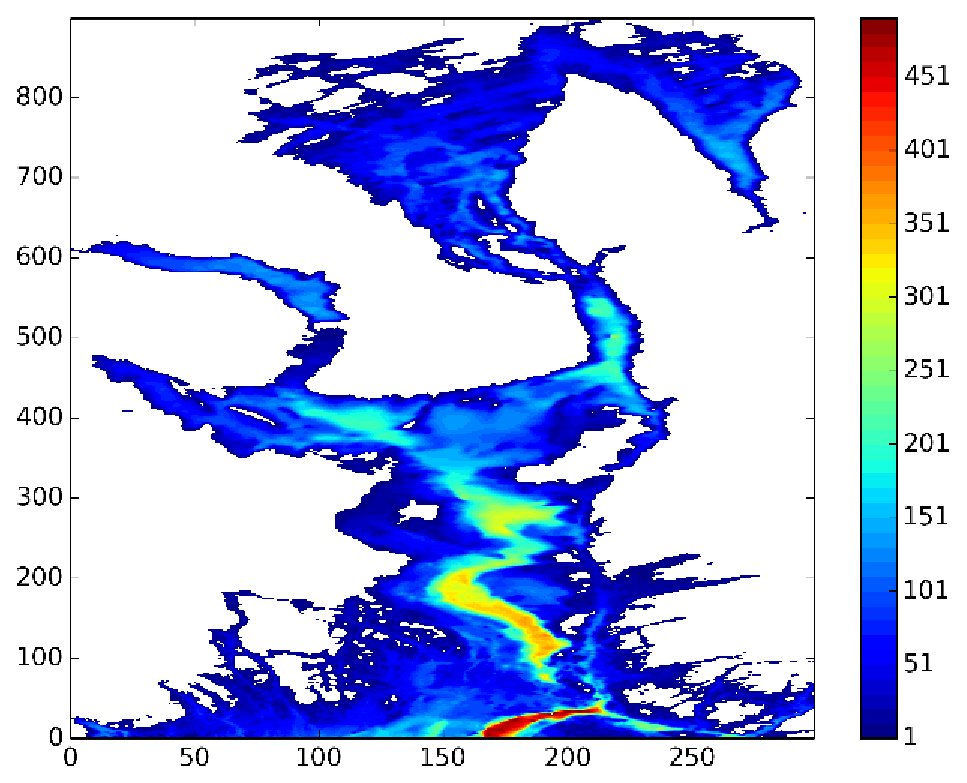
\includegraphics[height=10cm]{fjordos_cl}}
% Liggende
%   \rput[b]( 7.5,0.0){\includegraphics[angle=90,width=15.0cm,height=6.4865cm]{fjordos_roms}}
%   \rput[b]( 7.5,0.0){\includegraphics[height=8cm]{fjordos_roms}}
  \end{pspicture}
  \caption{\small The transformed curvilinear grid of the Oslofjord. The colors gives the depth in meters according to the color bar to the right. Model grid numbers associated with the curvilinear grid are given along the axes. There are 300 x 900 grid points.} 
  \label{fig:fjordos_cl}
 \end{center}
\end{figure}




 

%%%%%%%%%%%%%%%%%%%%%% Observations %%%%%%%%%%%%%%%%%%%%%%%%%%%%%%%%%%
\section{Results from test runs}
\label{sec:resul}
All the results shown below are derived by running FjordOs CL on the Vilje supercomputer at the Norwegian High Performance Computing facilities in Trondheim. We show results from a hindcast initialized from NorKyst800 on April 1st, 2014 and continued up to and including the month of December 2015. 
All inputs are as described in Section \ref{subsec:atmos}.
 
The results from the hindcast are further discussed and evaluated in some detail in an upcoming report \citep{hjelm:etal:2016}. Here we merely present snapshots of fields of currents, temperature, salinity and sea level so as to properly appreciate the level of details that the FjordOs CL model provides. In this we focus on six areas, namely the Inner Oslofjord, the Drammensfjord, the {\DR} area (henceforth {\DR}), the mid part of the Oslofjord (henceforth Slagen), the outer western part (henceforth Tristein) and the outer eastern part of the Oslofjord (henceforth Hvaler). 

\subsubsection{Currents}
 %%%%%%%%%%%%%%%%%%% Figure  %%%%%%%%%%%%%%%
\begin{figure}[t]
  \begin{pspicture}(0,0)(15,12)
% Include graphs
	\rput[b](7.5,0){\includegraphics[height=12cm]{kap5/ferder1__0_current_crop}}
  \end{pspicture}
  \caption{\small  Currents .  }
  \label{fig:curr_oslo}
\end{figure}

  
 %%%%%%%%%%%%%%%%%%% Figure  %%%%%%%%%%%%%%%
\begin{figure}[b]
  \begin{pspicture}(0,0)(15,16)
% Include graphs
	\rput[b](7.5,0){\includegraphics[height=16cm]{kap5/ferder2__0_current_crop}}
  \end{pspicture}
  \caption{\small  As Figure \ref{fig:curr_oslo}, but for the Dr{\o}bak Sound and Vestfjorden area.}
  \label{fig:curr_drobak}
\end{figure}

  
 %%%%%%%%%%%%%%%%%%% Figure  %%%%%%%%%%%%%%%
\begin{figure}[t]
  \begin{pspicture}(0,0)(15,13)
% Include graphs
	\rput[bl](-0.5,0){\includegraphics[height=13cm]{kap5/drammen1__0_current_crop}}
	\rput[br](15.2,0){\includegraphics[height=13cm]{kap5/ferder3__0_current_crop}}
  \end{pspicture}
  \caption{\small  As Figure \ref{fig:curr_oslo}, but for the Drammensfjord left) and southern part of the Dr{\o}bak Sound and Breiangen area. Note the swift currents through narrow and shallow sound in the Svelvik area.}
  \label{fig:curr_breiangen}
\end{figure}

  
 %%%%%%%%%%%%%%%%%%% Figure  %%%%%%%%%%%%%%%
\begin{figure}[t]
  \begin{pspicture}(0,0)(15,12)
% Include graphs
	\rput[b](7.5,0){\includegraphics[height=12cm]{kap5/ferder4__0_current_crop}}
  \end{pspicture}
  \caption{\small  Currents Mefjordbaaen area.  }
  \label{fig:curr_mefjord}
\end{figure}

  
 %%%%%%%%%%%%%%%%%%% Figure  %%%%%%%%%%%%%%%
\begin{figure}[t]
  \begin{pspicture}(0,0)(15,12)
% Include graphs
	\rput[b](7.5,0){\includegraphics[height=12cm]{kap5/ferder5__0_current_crop}}
  \end{pspicture}
  \caption{\small  Currents Faerder area.  }
  \label{fig:curr_faerder}
\end{figure}

  
 %%%%%%%%%%%%%%%%%%% Figure  %%%%%%%%%%%%%%%
\begin{figure}[t]
  \begin{pspicture}(0,0)(15,14)
% Include graphs
	\rput[b](7.5,0){\includegraphics[height=14cm]{kap5/drammen1__0_current_crop}}
  \end{pspicture}
  \caption{\small  As for figure \ref{fig:curr_oslo}, but for the Drammensfjord and western Breidangen area.  }
  \label{fig:curr_drammen}
\end{figure}

  

\subsubsection{Temperature}
 %%%%%%%%%%%%%%%%%%% Figure  %%%%%%%%%%%%%%%
\begin{figure}[t]
  \begin{pspicture}(0,0)(15,12)
% Include graphs
	\rput[b](7.5,0){\includegraphics[height=12cm]{kap5/temp_hele_0_current_crop}}
  \end{pspicture}
  \caption{\small Sea surface temperature (SST) for the entire model domain of the FjordOs model. Note the high SST in the Drammensfjorden area. We believe this is most likely caused by the entrainment (mixing) of warmer water from below. This warm water is probably left from imperfect initial conditions. }
  \label{fig:temp_hele}
\end{figure}

  

\subsubsection{Salinity}
 %%%%%%%%%%%%%%%%%%% Figure  %%%%%%%%%%%%%%%
\begin{figure}[t]
  \begin{pspicture}(0,0)(15,12)
% Include graphs
	\rput[b](7.5,0){\includegraphics[height=12cm]{kap5/salt_hele_0_current_crop}}
  \end{pspicture}
  \caption{\small  Salinity.  }
  \label{fig:salt_hele}
\end{figure}

  

\subsubsection{Sea level}
 %%%%%%%%%%%%%%%%%%% Figure  %%%%%%%%%%%%%%%
\begin{figure}[t]
  \begin{pspicture}(0,0)(15,12)
% Include graphs
	\rput[b](7.5,0){\includegraphics[height=12cm]{kap5/zeta_hele_0_crop}}
  \end{pspicture}
  \caption{\small  As for figure \ref{fig:temp_hele}, but for sea surface height (SSH).  }
  \label{fig:ssh_hele}
\end{figure}

  


%%%%%%%%%%%%%%%%%%%%%% Model results %%%%%%%%%%%%%%%%%%%%%%%%%%%%%%%%%
\input{evalu.tex}

%%%%%%%%%%%%%%%%%%%%%% Summary and conclusions %%%%%%%%%%%%%%%%%%%%%%%
\newpage
\section{Summary and final remarks}
\label{sec:summa}
A documentation of a new Oslofjord model is provided. The new Oslofjord model, named FjordOs CL, is based on the publically available ocean model ROMS \citep{shche:mcwil:2005,shche:mcwil:2009,haidv:etal:2008}, and is developed as part of the project FjordOs. FjordOs CL exploits the curvilinear option in ROMS to minimize the number of ``dry'' grid points at the expense of increasing the number of ``wet'' grid points. Thereby the grid resolution is enhanced and varies in space. In fact, the FjordOs CL mesh size varies from about 50 m in the {\DR} area to about 300 m at its southern border. 

To satisfy ourselves that the model works technically, is viable and produces results that are in line with our knowledge of the circulation in the fjord, we have run several test cases. Above we have shown examples of results from a hindcast case initiated on April 1, 2014 and run through December 31, 2015. A through validation of the results from this hindcast will be reported in a separate report.

In summary the results shown provides insight into the necessity of resolving the Oslofjord's irregular coastline geography, that is, the fjord's many small islands, narrow sounds and straits, and its topography, that is, deep basins and shallow areas. Thus, the new model provides a basis for developing an operation Oslofjord model once well identified and validated.


%\section*{Acknowledgement}
\addcontentsline{toc}{section}{Acknowledgement}
\input{acknow.tex}

%%% LPR: Added a specification where to find the path to the bibtex 
%        reference file. Needed when using the package natbib. 
%\bibliography{references}

\addcontentsline{toc}{section}{References}
\bibliography{$HOME/LATEX/bib-files/referanse-lpr.bib}
%\bibliography{referanse-lpr.bib}

%\clearpage
%\section*{Appendix}

%%%%%%%%%%%%%%%%%%%%%% Tables %%%%%%%%%%%%%%%%%%%%%%%%%%%%%%%%%%%%%%%%
%\clearpage
%\addcontentsline{toc}{section}{Tables}
%\input{table.tex}

%\begin{table}[h]
%\vspace{-1.5cm}
%{\bf Table A1: ESD statistics.}\\
%\label{tab:1}
%\begin{tabular}{llll}
%\small OSLO - BLINDERN 18700 & 
%\small $T_m$ $R^2$= 71 -- 86 $T_x$ $R^2$= 69 -- 82 $T_n$ $R^2$= 49 -- 76 \\
%\small $\Delta T_m$ $q_{0.05}$= 3.21 $q_{0.50}$= 1.33 $q_{0.95}$= 1.75 \\  
%\small $\Delta T_x$ $q_{0.05}$= 3.09 $q_{0.50}$= 1.38 $q_{0.95}$= 2.16 \\  
%\small $\Delta T_n$ $q_{0.05}$= 3.15 $q_{0.50}$= 1.12 $q_{0.95}$= 1.01 \\
%\end{tabular}
%\end{table}

%%%%%%%%%%%%%%%%%%%%%% Figures %%%%%%%%%%%%%%%%%%%%%%%%%%%%%%%%%%%%%%%
\clearpage
\addcontentsline{toc}{section}{Figures}
\input{figur.tex} 

%\clearpage
%\pagebreak

%\bibliography{refs}

%\clearpage
%\pagebreak
 

\end{document}



